\subsection{Trace-label audit}

Figure~\ref{fig:trace} reports the final-aligned trace counts. Its path labels identify where recorded state changed, not which loop alone caused the final outcome. A residual specification-side label likewise records semantic evidence such as a weak accepted specification or unresolved obligation, whereas an implementation-side label requires sufficiently clear contract and verifier evidence.

A balanced 36-sample audit evaluates this distinction (Table~\ref{tab:audit}). It contains 12 solved and 12 system-labeled spec-side samples, together with 12 implementation-side samples supplemented from auxiliary ablations because only four such residual labels appear in the full final-aligned run. The reviewer examines the raw task, accepted specification, final code, latest verifier signal, and system label. Strict agreement is 58.3\% (21 of 36), with one additional partial match for 61.1\% relaxed agreement. The accepted specification is judged fully adequate in 25 cases and partially adequate in 7 more, yielding 88.9\% combined adequacy.

\begin{table}[t]
\centering
\small
\begin{tabular}{@{}lrrrr@{}}
\toprule
Trace label & $n$ & Agree \up & Partial & Disagree \down \\
\midrule
Solved & 12 & 12 & 0 & 0 \\
Spec-side & 12 & 1 & 1 & 10 \\
Impl.-side & 12 & 8 & 0 & 4 \\
Overall & 36 & 21 & 1 & 14 \\
\bottomrule
\end{tabular}
\caption{Human audit of trace-based attribution labels.}
\label{tab:audit}
\end{table}

All 12 solved labels agree with the audit, and 8 of 12 implementation-side labels are confirmed. Spec-side labels are less precise: one is confirmed and one partially matches.

\subsection{Case study}
\label{app:case-study}

\begin{figure}[H]
\centering
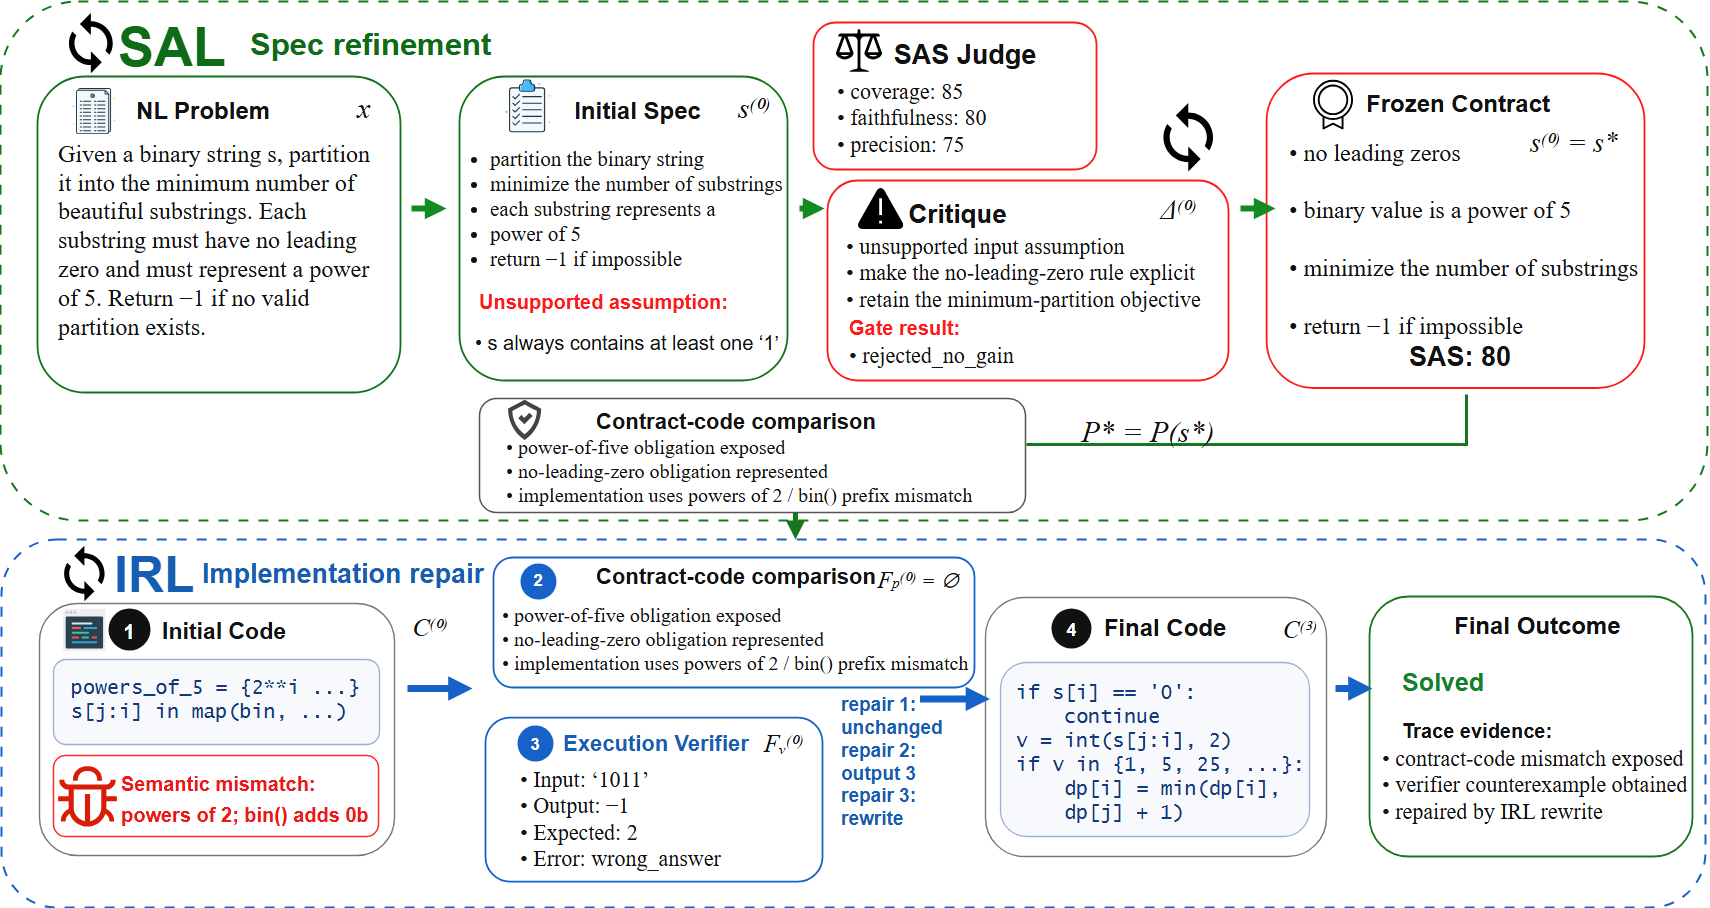
\includegraphics[width=\linewidth]{pics/case_study_cn.png}
\caption{Case-study trace for LiveCodeBench problem 2883.}
\label{fig:case}
\end{figure}

Figure~\ref{fig:case} explains one trace rather than adding an aggregate result. The upper SAL band judges, gates, and freezes the semantic target before implementation, and the lower IRL band checks and repairs code under that target. The task seeks a minimum partition of a binary string into powers of five with no leading zero. Initial $s^{(0)}$ already records the power-of-five condition, no-leading-zero rule, minimum objective, and $-1$ fallback. The judge assigns $q^{(0)}=(85,80,75)$ and, as the aggregate returned under the rubric rather than a recomputed weighted sum, $\mathrm{SAS}^{(0)}=80$; it then proposes a local clarification. Rejudging merged candidate $\hat{s}^{(1)}$ produces no gain, so $\mathrm{Improve}^{(1)}=0$ and the gate rejects it. SAL retains $s^{(0)}$, terminates, and directly freezes that current state: $s^\star=s^{(0)}$ and $\mathrm{SAS}(x,s^\star)=80$. No additional specification variant is generated or selected.

The bridge $P^\star=P(s^\star)$ marks the compiled subset; the contract--code comparison boxes are explanatory, not feedback variables. Initial $C^{(0)}$ constructs powers with \texttt{2**i} and compares substrings with \texttt{bin()} strings retaining the \texttt{0b} prefix.

Feedback $F_v^{(0)}$ exposes the mismatch: for \texttt{"1011"}, the program returns $-1$, while \texttt{"101"}\,$|$\,\texttt{"1"} gives 2. IRL converts substrings with \texttt{int(substring,2)}, checks powers-of-five membership, enforces no leading zero, and updates the dynamic program. Since $F_p^{(0)}=\emptyset$, verifier-guided repair receives credit for this transition. The contract makes the obligation legible; $F_v$ drives the correction.
